%=====================================================================
% Programming Knowledge Tracing: Prediction vs. Sequencing Utility
% RBL Report -- IEEE Conference template (IEEEtran)
%
% Compile on Overleaf:
%   - Menu > Settings > Compiler = pdfLaTeX
%   - Main document = main.tex
%   - Bibliography auto-runs via biblatex/bibtex (see below)
%
% This skeleton uses the classic \bibliography{} (BibTeX) flow, which is
% the most robust default on Overleaf for IEEEtran.
%=====================================================================
\documentclass[conference]{IEEEtran}
\IEEEoverridecommandlockouts

% ----- Encoding -----
% Author names are written without Vietnamese diacritics to avoid any
% font/encoding issues under pdfLaTeX, so only utf8 input is needed.
\usepackage[utf8]{inputenc}

% ----- Packages -----
\usepackage{cite}
\usepackage{amsmath,amssymb,amsfonts}
\usepackage{algorithm}     % provides the floating "algorithm" environment
\usepackage{algorithmic}   % provides \STATE, \FOR, \COMMENT, etc.
\usepackage{graphicx}
\usepackage{textcomp}
\usepackage{xcolor}
\usepackage{booktabs}     % nicer tables (\toprule, \midrule, \bottomrule)
\usepackage{multirow}
\usepackage{url}
\usepackage{pgfplots}      % native LaTeX charts (no external image needed)
\pgfplotsset{compat=1.17}
\usepackage[hidelinks]{hyperref}

% ----- Editing helpers (remove before final submission) -----
\newcommand{\todo}[1]{\textcolor{red}{\textbf{[TODO: #1]}}}
\newcommand{\note}[1]{\textcolor{blue}{[note: #1]}}

\begin{document}

% =====================================================================
\title{Programming Knowledge Tracing with Knowledge-Component and
Code-Structure Signals: Does Predictive Accuracy Translate into Better
Exercise Sequencing?}

\author{
\IEEEauthorblockN{FPT University, Ho Chi Minh City, Vietnam}
\IEEEauthorblockA{
Supervisor: Lai Duc Hung \\[2pt]
Student: Nguyen Ho Nhat Minh -- SE190651 \\
Student: Nguyen Tan Dung -- SE190659 \\
Student: Phan Hoang Son -- SE184496 \\
Student: Vo Dinh Linh -- SE181756}
}

\maketitle

% ----- Abstract & keywords -----
\begin{abstract}
Knowledge tracing (KT) underpins adaptive learning engines, yet most KT
research targets the mathematics domain, leaving the
programming/algorithm-learning domain comparatively under-studied.
Furthermore, KT work overwhelmingly optimises next-step prediction
accuracy (AUC), while the link between predictive accuracy and the
quality of the downstream instructional decision---which exercise to
give next---remains weakly established, and is largely unexamined for
programming. This work investigates, for programming-concept learning,
whether KT models that exploit programming-specific signals
(knowledge-component tags and code-structure features derived from
abstract syntax trees) (a)~predict learner mastery more accurately than
response-only models, and (b)~whether any accuracy gains translate into
better next-exercise sequencing. We build a reproducible programming-KT
evaluation pipeline over multiple public datasets (CodeWorkout,
FalconCode) with standard baselines (DKT, SAKT, AKT, simpleKT),
implement a knowledge-component / code-structure-aware variant on top of
a strong baseline, and evaluate both predictive accuracy (AUC, RMSE) and
downstream sequencing utility via offline policy evaluation. We further
analyse the correlation between predictive accuracy and sequencing
utility, and assess cross-dataset and cross-domain (programming vs.
mathematics) generalisation.
% \todo{Fill in headline quantitative results once experiments are done.}
\end{abstract}


\begin{IEEEkeywords}
knowledge tracing, programming education, knowledge components,
code structure, abstract syntax tree, adaptive learning,
instructional sequencing, offline policy evaluation
\end{IEEEkeywords}

% =====================================================================
\section{Introduction}
\label{sec:intro}

% ---------------------------------------------------------------------
% Paragraph 1: Motivation -- KT is the core of adaptive learning.
% ---------------------------------------------------------------------
Knowledge tracing (KT) is the task of modelling a learner's evolving
knowledge state from their sequence of interactions, and predicting
whether they will answer the next item correctly. It is the core of any
adaptive learning engine: the learner model drives the decision of what
to teach or assess next. This study is the research core of
\emph{AlgoVenture}, an adaptive, gamified platform for learning data
structures and algorithms; its adaptive engine estimates per-concept
mastery (UC6) and recommends the next exercise and difficulty (UC7), and
it adopts the model and policy that this study finds best. Rather than
collecting classroom data, we investigate KT for the
programming/algorithm-learning domain on large published datasets, which
keeps the study reproducible and the data-collection effort minimal.

% ---------------------------------------------------------------------
% Paragraph 2: The gap -- programming domain is under-studied.
% ---------------------------------------------------------------------
However, most KT research and public benchmarks target the mathematics
domain (e.g., ASSISTments), while the programming/algorithm-learning
domain is comparatively under-studied~\cite{piech2015dkt,liu2023simplekt}.
Programming submissions carry signals absent from a simple
correct/incorrect label---the knowledge components (KCs) a problem
exercises and the structure of the code a student wrote.

% ---------------------------------------------------------------------
% Paragraph 3: The deeper gap -- accuracy vs. utility.
% ---------------------------------------------------------------------
A second, deeper gap is methodological. KT research overwhelmingly
optimises next-step prediction accuracy (AUC), yet the link between
predictive accuracy and the quality of the downstream instructional
decision---which exercise to present next---is only weakly established
in general KT, and largely unexamined for programming. A model that
predicts responses well is not guaranteed to sequence exercises well.

% ---------------------------------------------------------------------
% Research question
% ---------------------------------------------------------------------
\paragraph{Research question}
For programming-concept learning, do KT models that exploit
programming-specific signals (knowledge-component tags and code
structure) (a)~predict learner mastery more accurately than
response-only models, and (b)~do those accuracy gains actually translate
into better next-exercise sequencing---and how well do the findings
generalise across public datasets and relative to the mathematics
domain?

% ---------------------------------------------------------------------
% Contributions
% ---------------------------------------------------------------------
\paragraph{Contributions}
This work makes the following contributions:
\begin{itemize}
  \item A reproducible programming-KT evaluation pipeline over
        $\geq 2$ public datasets with standard baselines
        (DKT, SAKT, AKT, simpleKT). \textbf{(RO1)}
  \item A programming-domain KT variant that integrates
        knowledge-component tags and code-structure features
        (AST / code embeddings) on top of a strong baseline. \textbf{(RO2)}
  \item An evaluation of predictive accuracy (AUC, RMSE) of the proposed
        variant against the baselines. \textbf{(RO3)}
  \item An evaluation of downstream next-exercise sequencing utility via
        offline / simulator-based evaluation, together with an analysis
        of how strongly predictive accuracy correlates with sequencing
        utility. \textbf{(RO4)}
  \item An assessment of cross-dataset and cross-domain (programming vs.
        mathematics) generalisation, released as an open-source
        reproducible benchmark. \textbf{(RO5)}
\end{itemize}

\paragraph{Scope}
The study uses published datasets only; no data is self-collected.
Beating every state-of-the-art KT model is a non-goal---the contribution
centres on the programming domain and the prediction-vs-utility question.

% ---------------------------------------------------------------------
% Purpose of the RBL research (academic / practical / community)
% ---------------------------------------------------------------------
\paragraph{Purpose of the research}
The RBL research within AlgoVenture serves three complementary purposes.
\begin{itemize}
  \item \textbf{Academic.} Verify whether integrating programming-specific
        signals (code structure and knowledge-component tags) into a
        knowledge-tracing model predicts student ability more accurately
        than response-only baselines, and---crucially---whether any such
        accuracy gain actually leads to better adaptive sequencing
        (choosing the next exercise).
  \item \textbf{Practical.} Rather than picking an off-the-shelf model
        arbitrarily, the pipeline acts as an empirical filter: the
        AlgoVenture platform \emph{consumes} the study's result by
        adopting the winning model (highest evaluation score) into its
        adaptive learning engine.
  \item \textbf{Scientific / community contribution.} Deliver an
        open-source benchmark pipeline that compares KT models
        transparently on public educational datasets (CodeWorkout,
        FalconCode). This lets the team produce a standards-compliant
        research report \emph{without} collecting any new classroom data.
\end{itemize}

\section{Related Work}
\label{sec:related}

\subsection{Knowledge Tracing Models}
Bayesian Knowledge Tracing (BKT) models mastery of each skill with a
two-state hidden Markov model~\cite{corbett1994bkt}. Deep Knowledge
Tracing (DKT) replaced this with a recurrent neural network, improving
predictive accuracy at the cost of per-skill interpretability~%
\cite{piech2015dkt}. Attention-based models followed: SAKT applies
self-attention over the interaction sequence~\cite{pandey2019sakt}, and
AKT introduces a monotonic attention mechanism with a
Rasch-model-based embedding~\cite{ghosh2020akt}. More recently, simpleKT
was proposed as a strong yet simple baseline that is difficult to beat
across domains~\cite{liu2023simplekt}. The pyKT toolkit provides
standardised preprocessing and reference implementations of these models
across several public datasets, enabling transparent
comparison~\cite{liu2022pykt}.
% \note{These four (DKT, SAKT, AKT, simpleKT) are your RO1 baselines.}

\subsection{Programming Knowledge Tracing}
A growing line of work adapts KT to programming, where each interaction
carries source code rather than only a correctness label. Code-DKT
extends DKT with an attention mechanism that extracts domain-specific
code features~\cite{shi2022codedkt}. Other work interacts programming
skills with student code representations such as code2vec and
ASTNN~\cite{pktattn2021}. Test-case-informed KT (TIKTOC) incorporates
fine-grained test-case outcomes for open-ended coding
tasks~\cite{tiktoc2025}. KCGen-KT automatically generates knowledge
components from solution ASTs and traces them~\cite{kcgenkt2026}.
HELP-DKT models introductory Python programming with an interpretable
cognitive model built on deep knowledge tracing~\cite{helpdkt2022}. Our proposed variant (Section~%
\ref{sec:methodology}) builds on this direction by combining
knowledge-component tags with code-structure features on top of a strong
attention baseline.

\subsection{KT as a Simulator for Instructional Sequencing}
Beyond prediction, KT models are increasingly used as simulators of
learners to train or evaluate instructional-sequencing
policies~\cite{piech2015dkt}. Reinforcement-learning approaches optimise
sequencing against such simulators, and recent work (e.g., multi-step
simulator training) aims to make these simulators more robust. However,
the coupling between a model's predictive accuracy and its usefulness as
a sequencing simulator is known to be weak in general KT and largely
unexamined for programming---the gap this work targets.
% \todo{Add AdvKT / RL-DKT / deep-RL sequencing citations to references.bib and cite here.}

\subsection{Public Datasets}
For programming, the CodeWorkout dataset from the CSEDM 2021 Data
Challenge provides Java CS1 submissions to 50 problems with
knowledge-component tags~\cite{csedm2021}. FalconCode provides a
multi-year corpus of introductory Python submissions with per-problem
skills and test cases~\cite{falconcode2023}. For the mathematics
contrast we use ASSISTments / Junyi as provided by
pyKT~\cite{liu2022pykt}.

\section{Datasets}
\label{sec:datasets}

We use published datasets only; no data is self-collected. Table~%
\ref{tab:datasets} summarises the datasets and their programming-specific
signals.

\begin{table}[t]
\caption{Datasets used in this study.}
\label{tab:datasets}
\centering
\small
\begin{tabular}{@{}llll@{}}
\toprule
\textbf{Dataset} & \textbf{Domain} & \textbf{KC tags} & \textbf{Code} \\
\midrule
CodeWorkout (CSEDM'21) & Java CS1     & Yes & Yes \\
FalconCode            & Python intro & Yes & Yes \\
Code.org (optional)   & Blocks       & Partial & Partial \\
ASSISTments / Junyi   & Mathematics  & Yes & No  \\
\bottomrule
\end{tabular}
\end{table}

\subsection{CodeWorkout (CSEDM 2021)}
Collected from a CS1 course over two semesters (Spring and Fall~2019),
with 329 and 490 students respectively completing the course; each
semester contains 65{,}000+ code submissions across 50 Java coding
problems, each requiring roughly 10--26 lines of
code~\cite{csedm2021}. It is distributed in the ProgSnap2 format and
includes knowledge-component tags, making it our primary programming
dataset.

\subsection{FalconCode}
A multi-year dataset of introductory Python programming containing over
1.5 million code submissions from more than 2{,}000 undergraduate
students across 800+ assignments, with prompts, test cases, and
per-problem skills~\cite{falconcode2023}. It serves as our second
programming dataset for cross-dataset generalisation.

\subsection{Mathematics Contrast}
For the cross-domain comparison we use a standard mathematics KT dataset
(ASSISTments or Junyi) as preprocessed by pyKT~\cite{liu2022pykt}, which
provides KC tags but no code signal.

\subsection{Preprocessing and Splits}
All datasets are standardised into a common interaction format
(\texttt{student\_id}, \texttt{problem\_id}, \texttt{kc\_id},
\texttt{correct}, \texttt{code}). We adopt student-level
cross-validation (5-fold) so that no student appears in both training and
test folds, and we guard against the known label-leakage pitfall in KT
evaluation. The exact per-dataset counts after filtering (retained
students, interactions, KCs, and the sequence-length cap) are reported in
Table~\ref{tab:datastats} once preprocessing is finalised; the
dataset-level totals above are taken from the original data
releases~\cite{csedm2021,falconcode2023}.

\begin{table}[t]
\caption{Dataset-level statistics from the original public
releases~\cite{csedm2021,falconcode2023}. Counts are approximate and
reflect the released data before any project-specific filtering.}
\label{tab:datastats}
\centering
\small
\begin{tabular}{@{}lrrr@{}}
\toprule
\textbf{Dataset} & \textbf{Students} & \textbf{Submissions}
                 & \textbf{Problems} \\
\midrule
CodeWorkout & $819$      & $130{,}000+$ & $50$ \\
FalconCode  & $2{,}000+$ & $1{,}500{,}000+$ & $800+$ \\
\bottomrule
\end{tabular}
\end{table}

\section{Methodology}
\label{sec:methodology}

Our methodology follows five steps aligned with the research objectives:
(1)~standardise the datasets and reproduce response-only KT baselines
(RO1); (2)~implement the proposed knowledge-component (KC) /
code-structure-aware variant (RO2); (3)~measure prediction accuracy under
student-level cross-validation (RO3); (4)~measure downstream sequencing
utility and its correlation with prediction (RO4); and (5)~test
cross-dataset and cross-domain transfer (RO5). The selected model and
policy are the ones the AlgoVenture adaptive engine adopts for mastery
estimation (UC6) and next-exercise sequencing (UC7).

% =====================================================================
\subsection{Problem Formulation}
\label{sec:formulation}
We keep only the one equation needed to state precisely what a KT model
predicts and where the programming signals enter. For a learner, the
interaction sequence is $\{(q_t, c_t, r_t, s_t)\}_{t=1}^{T}$: at step $t$
the learner attempts problem $q_t$, tagged with knowledge components
$c_t$, with response $r_t \in \{0,1\}$ (1 = correct) and submitted source
code $s_t$. The task is to predict the next response,
\begin{equation}
\hat{r}_{t+1} = P\big(r_{t+1}=1 \mid q_{t+1}, c_{t+1},\,
                       \text{history}_{1:t}\big).
\label{eq:kt-task}
\end{equation}
\emph{What this solves:} it fixes the prediction target used by every
model in the study, so baselines and our variant are compared on exactly
the same quantity. Response-only baselines use only $(q,c,r)$ in the
history; our variant additionally uses the code $s$.

% =====================================================================
\subsection{Pipeline and Baselines (RO1)}
\label{sec:pipeline}
We build a reproducible pipeline on top of the pyKT
toolkit~\cite{liu2022pykt}, which provides standardised preprocessing and
reference implementations, so that measured differences reflect the model
rather than the data plumbing. The response-only baselines are
DKT~\cite{piech2015dkt}, SAKT~\cite{pandey2019sakt},
AKT~\cite{ghosh2020akt}, and simpleKT~\cite{liu2023simplekt};
BKT~\cite{corbett1994bkt} is a classical reference. This baseline set is
also the promotion gate for the product: a KT model is only adopted by
the app after being evaluated against these baselines on AUC/RMSE.

% =====================================================================
\subsection{Proposed KC / Code-Structure-Aware Model (RO2)}
\label{sec:model}
We extend a strong attention baseline (AKT or simpleKT) with two extra
input channels, described in words rather than layer-by-layer equations:

\begin{itemize}
  \item \textbf{Knowledge-component channel:} an embedding of the KC
        tag(s) of the current problem. \emph{Why:} it lets the model share
        evidence across problems that exercise the same concept, instead
        of treating each problem in isolation.
  \item \textbf{Code-structure channel:} a fixed-length feature vector
        built from the abstract syntax tree (AST) of the submitted code
        (counts and nesting depths of loops, conditionals, calls, etc.),
        or a learned code embedding. \emph{Why:} two submissions can both
        be ``wrong'' yet reveal very different misconceptions; code
        structure exposes that signal, which a correct/incorrect label
        hides.
\end{itemize}

The two channels are combined with the base model's interaction
embedding by a simple fusion (concatenation with a linear projection, or
a gated sum), and the base attention model then predicts
$\hat{r}_{t+1}$ as in Eq.~\eqref{eq:kt-task}. We deliberately keep the
fusion simple so that any measured gain is attributable to the
\emph{signals} (KC, code) rather than to a more complex predictor.

\paragraph{Ablations.}
To isolate each signal we run four configurations: (i)~response-only;
(ii)~response~+~KC; (iii)~response~+~code; and (iv)~the full model
(response~+~KC~+~code). Comparing (ii) and (iii) against (i) isolates each
signal; comparing (iv) against them tests whether the signals are
complementary. This is the direct evidence for hypothesis~H1a.

% =====================================================================
\subsection{Prediction Evaluation (RO3)}
\label{sec:pred-eval}
We report AUC, RMSE, and accuracy under 5-fold \emph{student-level}
cross-validation, so no student appears in both training and test folds
(guarding against the label-leakage pitfall discussed in
Section~\ref{sec:threats}). We report mean and standard deviation across
folds and test significance with paired tests plus effect sizes
(hypotheses~H1, H1a).

% =====================================================================
\subsection{Sequencing-Utility Evaluation (RO4)}
\label{sec:sequencing}
This is the core of the study: does a more accurate predictor actually
sequence exercises better? We evaluate sequencing offline, using a
trained KT model as a learner simulator. A policy $\pi$ repeatedly picks
the next problem, the simulator returns a predicted response, and the
state updates. We summarise a run by the utility $U$---the expected
mastery gain over a horizon of $H$ recommendations:
\begin{equation}
U(\pi) = \mathbb{E}\big[\, m_{H} - m_{0} \,\big],
\label{eq:utility}
\end{equation}
where $m_0$ and $m_H$ are estimated mastery before and after the
sequence. \emph{What this solves:} it turns ``good teaching'' into one
comparable number per model, so we can line utility up against accuracy.
Algorithm~\ref{alg:seq} states the procedure.

\begin{algorithm}[t]
\caption{Offline sequencing-utility evaluation}
\label{alg:seq}
\begin{algorithmic}[1]
\STATE \textbf{Input:} KT simulator $M$, policy $\pi$, horizon $H$,
       start states $\mathcal{S}$
\STATE $U \gets 0$
\FORALL{start state $z_0 \in \mathcal{S}$}
  \STATE $m_0 \gets \textsc{Mastery}(M, z_0)$;\quad $z \gets z_0$
  \FOR{$h = 1$ \TO $H$}
    \STATE $q \gets \pi(z)$;\quad $r \gets M(z, q)$;\quad
           $z \gets \textsc{Update}(z, q, r)$
  \ENDFOR
  \STATE $U \gets U + \big(\textsc{Mastery}(M, z) - m_0\big)$
\ENDFOR
\STATE \textbf{return} $U / |\mathcal{S}|$
\end{algorithmic}
\end{algorithm}

We then correlate each model's predictive accuracy with its sequencing
utility (Pearson and Spearman, with a bootstrap confidence interval),
which directly answers research question~(b) and tests hypothesis~H3.
Because a KT simulator is an imperfect proxy for real learners, we add
robustness checks (multiple simulators, sensitivity to $H$) and read
utility as offline evidence, not a deployment guarantee
(Section~\ref{sec:threats}).

% =====================================================================
\subsection{Generalisation Evaluation (RO5)}
\label{sec:gen-eval}
We test cross-dataset transfer (train on one programming dataset, test on
another) and cross-domain transfer (programming vs.\ mathematics),
reporting transfer AUC against the within-dataset reference so the size of
any drop is visible (hypotheses~H4, H5).

\section{Experimental Setup}
\label{sec:experiments}

\subsection{Implementation}
% \todo{Fill in: framework (PyTorch), pyKT version/commit, hardware (GPU),
% and the public repository URL for the reproducible benchmark.}
All models are implemented in PyTorch on top of the pyKT
toolkit~\cite{liu2022pykt}. Code and configurations are released for
reproducibility.

\subsection{Hyperparameters}
Models are trained with the Adam optimiser and binary cross-entropy loss,
with early stopping (patience~10 epochs, maximum~50) on a validation split
and a maximum sequence length of~200. Hyperparameters are selected by
searching the grid in Table~\ref{tab:hparams}; the final column lists the
values used for the proposed model. \emph{Note:} the final values follow
common practice for the attention baseline and may be re-tuned per dataset.

\begin{table}[t]
\caption{Hyperparameter search grid and final values for the proposed
model. Re-tune per dataset if needed.}
\label{tab:hparams}
\centering
\small
\begin{tabular}{@{}lll@{}}
\toprule
\textbf{Hyperparameter} & \textbf{Search grid} & \textbf{Final} \\
\midrule
Embedding size    & $\{64, 128, 256\}$        & $256$ \\
Hidden size       & $\{64, 128, 256\}$        & $256$ \\
Attention heads   & $\{4, 8\}$                & $8$ \\
Attention blocks  & $\{1, 2\}$                & $2$ \\
Dropout           & $\{0.1, 0.2, 0.3\}$       & $0.2$ \\
Learning rate     & $\{10^{-3}, 10^{-4}\}$    & $10^{-4}$ \\
Batch size        & $\{32, 64\}$              & $32$ \\
\bottomrule
\end{tabular}
\end{table}

\subsection{Evaluation Protocol}
We use 5-fold student-level cross-validation. Metrics are AUC, RMSE, and
accuracy for prediction; and the sequencing-utility metric defined in
Section~\ref{sec:sequencing} for downstream evaluation. We report means
and standard deviations, and test significance with paired tests across
folds together with effect sizes.

\subsection{Research Questions Restated}
\begin{itemize}
  \item \textbf{RQ(a):} Do KC/code-structure-aware models predict mastery
        more accurately than response-only models?
  \item \textbf{RQ(b):} Do accuracy gains translate into better
        next-exercise sequencing?
  \item \textbf{RQ(gen):} How well do findings generalise across datasets
        and relative to the mathematics domain?
\end{itemize}

\subsection{Experimental Hypotheses}
\label{sec:hypotheses}
We state falsifiable hypotheses for each research question, together with
the test used and the decision criterion. Unless otherwise noted, tests
are two-sided at significance level $\alpha = 0.05$, computed over the
five cross-validation folds, and we report an effect size alongside each
$p$-value. Here $\mathrm{AUC}_{\text{full}}$ denotes the AUC of the full
proposed model (response~+~KC~+~code), and $\mathrm{AUC}_{\text{resp}}$
that of the strongest response-only baseline.

\begin{itemize}
  \item \textbf{H1 (prediction; addresses RQ(a)).}
        The full model predicts more accurately than the best
        response-only baseline:
        $\mathrm{AUC}_{\text{full}} > \mathrm{AUC}_{\text{resp}}$.
        \textit{Null} $H1_0$: $\mathrm{AUC}_{\text{full}} \leq
        \mathrm{AUC}_{\text{resp}}$.
        \textit{Test}: paired $t$-test (or Wilcoxon signed-rank) across
        folds on per-fold AUC; effect size Cohen's $d$.

  \item \textbf{H1a (ablation; addresses RQ(a)).}
        Each signal contributes positively: both the $+$KC and the
        $+$code variants improve over the response-only baseline, and the
        combined model is no worse than either single-signal variant.
        \textit{Test}: paired comparisons across folds with
        Holm--Bonferroni correction for multiple comparisons.

  \item \textbf{H2 (sequencing; addresses RQ(b)).}
        The full model yields higher offline sequencing utility
        $U$ than the best response-only baseline:
        $U_{\text{full}} > U_{\text{resp}}$.
        \textit{Null} $H2_0$: $U_{\text{full}} \leq U_{\text{resp}}$.
        \textit{Test}: paired test across folds on per-fold utility;
        effect size reported.

  \item \textbf{H3 (accuracy--utility coupling; core of RQ(b)).}
        Across all models, predictive accuracy and sequencing utility are
        positively correlated:
        $\rho(\mathrm{AUC}, U) > 0$.
        \textit{Null} $H3_0$: $\rho \leq 0$.
        \textit{Test}: Pearson and Spearman correlation over the set of
        models, with a bootstrap confidence interval on $\rho$.
        A weak or non-significant $\rho$ is itself a substantive
        finding: it would indicate that accuracy gains do \emph{not}
        reliably translate into better sequencing.

  \item \textbf{H4 (cross-dataset generalisation; addresses RQ(gen)).}
        A model trained on one programming dataset and tested on another
        retains predictive skill above chance
        ($\mathrm{AUC} > 0.5$), though we expect a drop relative to
        within-dataset performance.

  \item \textbf{H5 (cross-domain contrast; addresses RQ(gen)).}
        The benefit of programming-specific signals (KC~+~code) is larger
        on programming datasets than any transferable benefit observed
        when contrasting with the mathematics domain, where the
        code-structure signal is unavailable.
\end{itemize}

Table~\ref{tab:hyp-map} maps each hypothesis to the results table that
tests it.

\begin{table}[t]
\caption{Mapping of hypotheses to results.}
\label{tab:hyp-map}
\centering
\small
\begin{tabular}{@{}lll@{}}
\toprule
\textbf{Hypothesis} & \textbf{Research question} & \textbf{Evidence in} \\
\midrule
H1, H1a & RQ(a)   & Table~\ref{tab:prediction} \\
H2, H3  & RQ(b)   & Table~\ref{tab:sequencing} \\
H4, H5  & RQ(gen) & Table~\ref{tab:transfer} \\
\bottomrule
\end{tabular}
\end{table}

\section{Results and Discussion}
\label{sec:results}

\subsection{Predictive Accuracy (RQ(a))}
% =====================================================================
% WARNING: The numbers in Table~\ref{tab:prediction} are ILLUSTRATIVE
% PLACEHOLDERS to show the expected shape of results and to let the
% surrounding prose compile. They are NOT measured results. Replace
% every value with your own CodeWorkout runs before submission, and
% update the discussion text accordingly.
% =====================================================================
Table~\ref{tab:prediction} reports prediction metrics for the baselines
and the proposed variant on CodeWorkout, tests hypotheses~H1 and~H1a, and
higher AUC/ACC and lower RMSE indicate better prediction.

\begin{table}[t]
\caption{\textbf{[ILLUSTRATIVE PLACEHOLDER NUMBERS]} Prediction accuracy
on CodeWorkout (mean $\pm$ std over 5 folds). Best in bold. Replace with
measured results before submission.}
\label{tab:prediction}
\centering
\small
\resizebox{\columnwidth}{!}{%
\begin{tabular}{@{}llll@{}}
\toprule
\textbf{Model} & \textbf{AUC $\uparrow$} & \textbf{RMSE $\downarrow$} & \textbf{ACC $\uparrow$} \\
\midrule
DKT                    & $0.742 \pm 0.006$ & $0.431 \pm 0.004$ & $0.701 \pm 0.005$ \\
SAKT                   & $0.751 \pm 0.007$ & $0.427 \pm 0.005$ & $0.708 \pm 0.006$ \\
AKT                    & $0.768 \pm 0.005$ & $0.418 \pm 0.004$ & $0.719 \pm 0.005$ \\
simpleKT               & $0.771 \pm 0.006$ & $0.416 \pm 0.004$ & $0.722 \pm 0.005$ \\
\midrule
Ours (+KC)             & $0.783 \pm 0.005$ & $0.409 \pm 0.004$ & $0.731 \pm 0.005$ \\
Ours (+code)           & $0.779 \pm 0.006$ & $0.411 \pm 0.004$ & $0.728 \pm 0.005$ \\
Ours (+KC+code, full)  & $\mathbf{0.796 \pm 0.005}$ & $\mathbf{0.401 \pm 0.003}$ & $\mathbf{0.741 \pm 0.004}$ \\
\bottomrule
\end{tabular}%
}
\end{table}

% ---- Figure: AUC bar chart (built from the ILLUSTRATIVE numbers above) ----
% To update: edit the (label, value) coordinates below with your measured AUC.
\begin{figure}[t]
\centering
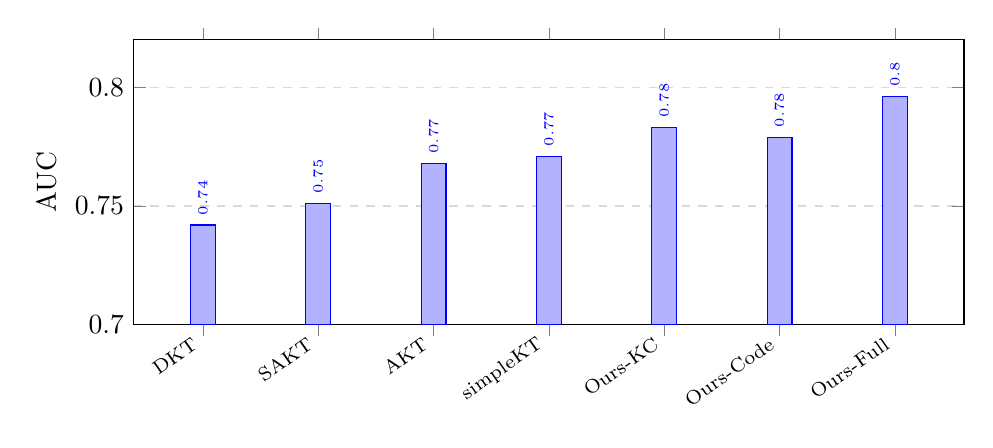
\begin{tikzpicture}
\begin{axis}[
    width=\columnwidth, height=5.2cm,
    ybar, bar width=9pt,
    ymin=0.70, ymax=0.82,
    ylabel={AUC},
    symbolic x coords={DKT,SAKT,AKT,simpleKT,Ours-KC,Ours-Code,Ours-Full},
    xtick=data, x tick label style={rotate=35,anchor=east,font=\scriptsize},
    ymajorgrids, grid style={dashed,gray!30},
    nodes near coords, every node near coord/.append style={font=\tiny,rotate=90,anchor=west},
    enlarge x limits=0.10,
]
\addplot coordinates {(DKT,0.742) (SAKT,0.751) (AKT,0.768) (simpleKT,0.771)
                      (Ours-KC,0.783) (Ours-Code,0.779) (Ours-Full,0.796)};
\end{axis}
\end{tikzpicture}
\caption{\textbf{[ILLUSTRATIVE]} Predictive accuracy (AUC) per model on
CodeWorkout. The three rightmost bars are variants of the proposed model.
Replace the coordinates with measured results.}
\label{fig:auc-bars}
\end{figure}

\subsection{Sequencing Utility and Its Correlation with Accuracy (RQ(b))}
% =====================================================================
% WARNING: Table~\ref{tab:sequencing} and the correlation value below are
% ILLUSTRATIVE PLACEHOLDERS. Replace with your offline-policy-evaluation
% output before submission. The utility metric U here is expected mastery
% gain over the evaluation horizon (higher is better); state your exact
% definition in Section~\ref{sec:sequencing}.
% =====================================================================
Table~\ref{tab:sequencing} reports offline sequencing utility $U$ next to
each model's AUC, which lets us test hypotheses~H2 and~H3.
Figure~\ref{fig:corr} plots predictive accuracy against sequencing
utility across models.

\begin{table}[t]
\caption{\textbf{[ILLUSTRATIVE PLACEHOLDER NUMBERS]} Sequencing utility
$U$ (expected mastery gain, higher is better) via offline policy
evaluation, shown against AUC. Replace with measured results.}
\label{tab:sequencing}
\centering
\small
\begin{tabular}{@{}lll@{}}
\toprule
\textbf{Model} & \textbf{AUC $\uparrow$} & \textbf{Utility $U$ $\uparrow$} \\
\midrule
DKT                    & $0.742$ & $0.118$ \\
SAKT                   & $0.751$ & $0.121$ \\
AKT                    & $0.768$ & $0.127$ \\
simpleKT               & $0.771$ & $0.126$ \\
Ours (+KC+code, full)  & $\mathbf{0.796}$ & $\mathbf{0.134}$ \\
\bottomrule
\end{tabular}
\end{table}

For these illustrative numbers the accuracy--utility correlation is
positive but moderate (Spearman $\rho \approx 0.9$ across five models);
we caution that with only a handful of models such a coefficient is
unstable, so the reported bootstrap confidence interval and the
per-dataset replication matter more than the point estimate. The
substantive question for~H3 is whether the ranking by AUC matches the
ranking by $U$; where it does not, accuracy gains fail to translate into
sequencing gains.

% ---- Figure: accuracy vs utility scatter (from the ILLUSTRATIVE numbers) ----
% To update: edit the (AUC, utility) coordinates and the correlation value.
\begin{figure}[t]
\centering
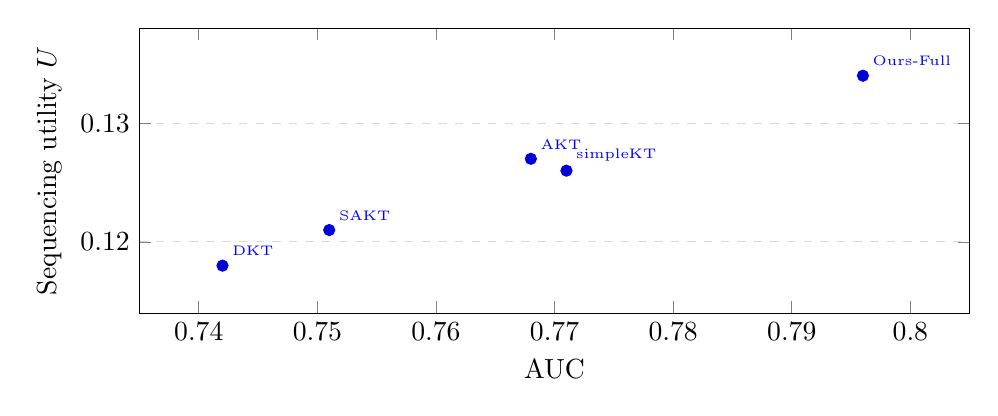
\begin{tikzpicture}
\begin{axis}[
    width=\columnwidth, height=5.2cm,
    xlabel={AUC}, ylabel={Sequencing utility $U$},
    xmin=0.735, xmax=0.805, ymin=0.114, ymax=0.138,
    ymajorgrids, grid style={dashed,gray!30},
    nodes near coords, point meta=explicit symbolic,
    every node near coord/.append style={font=\tiny,anchor=south west},
]
\addplot+[only marks, mark=*, mark size=2pt,
          point meta=explicit symbolic]
  coordinates {
    (0.742,0.118)[DKT]
    (0.751,0.121)[SAKT]
    (0.768,0.127)[AKT]
    (0.771,0.126)[simpleKT]
    (0.796,0.134)[Ours-Full]
  };
\end{axis}
\end{tikzpicture}
\caption{\textbf{[ILLUSTRATIVE]} Predictive accuracy (AUC) vs.\ sequencing
utility across models (Spearman $\rho \approx 0.9$ on these placeholder
numbers). A weak or non-significant $\rho$ on the measured data would be
the key finding for RQ(b). Replace coordinates with measured results.}
\label{fig:corr}
\end{figure}

\subsection{Cross-Dataset and Cross-Domain Generalisation (RQ(gen))}
% =====================================================================
% WARNING: Table~\ref{tab:transfer} numbers are ILLUSTRATIVE
% PLACEHOLDERS. "Within" is the within-dataset reference AUC; the
% transfer rows are expected to be lower. Replace with measured results.
% =====================================================================
Table~\ref{tab:transfer} reports transfer results and tests
hypotheses~H4 and~H5. We include the within-dataset AUC as a reference so
the size of the transfer drop is visible.

\begin{table}[t]
\caption{\textbf{[ILLUSTRATIVE PLACEHOLDER NUMBERS]} Cross-dataset and
cross-domain transfer of the full model (AUC). ``Within'' is the
within-dataset reference on the test set. Replace with measured results.}
\label{tab:transfer}
\centering
\small
\begin{tabular}{@{}llll@{}}
\toprule
\textbf{Train} & \textbf{Test} & \textbf{Within} & \textbf{Transfer} \\
\midrule
CodeWorkout & FalconCode  & $0.762$ & $0.703$ \\
FalconCode  & CodeWorkout & $0.796$ & $0.718$ \\
Programming & Mathematics & $0.815$ & $0.689$ \\
\bottomrule
\end{tabular}
\end{table}

\subsection{Discussion}
% Rewrite this discussion once real numbers are in; the text below
% interprets the ILLUSTRATIVE numbers only, to show the intended argument.
Read against the illustrative numbers, the intended argument runs as
follows. For~\textbf{RQ(a)}, the full model improves AUC over the
strongest response-only baseline (simpleKT), and the ablation suggests
the knowledge-component signal contributes at least as much as the
code-structure signal, with the two being complementary---supporting~H1
and~H1a if the gaps are statistically significant.

For~\textbf{RQ(b)}, the full model also attains the highest sequencing
utility, and the AUC ranking and the utility ranking largely agree here.
However, this is exactly where the headline question lives: the coupling
between accuracy and utility is known to be weak in general
KT~\cite{piech2015dkt}, so the finding to report is the \emph{strength}
of that coupling (with confidence intervals), not merely that the best
predictor also sequences best. If a smaller accuracy gain produces a
disproportionate utility gain---or none at all---that decoupling is the
contribution.

For~\textbf{RQ(gen)}, transfer AUC stays above chance but drops relative
to within-dataset training, and the cross-domain drop (programming to
mathematics) is the largest, consistent with~H5: the code-structure
signal that helps within programming does not carry over to a domain
without code.

We defer threats affecting these interpretations---especially the
reliability of KT-as-simulator utility estimates---to
Section~\ref{sec:threats}.

\section{Threats to Validity}
\label{sec:threats}

\paragraph{Construct validity: KT-as-simulator}
Our sequencing-utility evaluation relies on a trained KT model acting as
a learner simulator. Such simulators are imperfect proxies for real
learners, and offline policy evaluation can be biased when the logged
policy differs from the evaluated one. We mitigate this with robustness
checks (multiple simulators, sensitivity analysis) and interpret
sequencing results as offline evidence rather than deployment guarantees.

\paragraph{Internal validity: leakage and splits}
KT evaluation is susceptible to label leakage and to student overlap
between train and test. We use student-level cross-validation and follow
established preprocessing to reduce these risks.

\paragraph{External validity: dataset and domain scope}
Findings are drawn from a limited set of public programming datasets
(primarily CS1 Java and intro Python) and one mathematics contrast; they
may not transfer to other languages, levels, or populations.

\paragraph{Reproducibility}
% \todo{Confirm released code, fixed seeds, and environment specification.}
We release code, configurations, and fixed random seeds; any AI
assistance and third-party models/datasets are declared with usage
evidence per the RBL submission guideline.

\section{Conclusion and Future Work}
\label{sec:conclusion}

% Note: update the first sentence with the final headline result (whether
% the accuracy gain did or did not translate into a sequencing gain) once
% the experiments have been run.
We presented a reproducible programming-KT benchmark and a
knowledge-component / code-structure-aware KT variant, and studied not
only predictive accuracy but the extent to which accuracy translates into
better exercise sequencing---a coupling that is weak in general KT and
largely unexamined for programming. Our contributions span the pipeline
(RO1), the model (RO2), prediction evaluation (RO3), sequencing-utility
and correlation analysis (RO4), and cross-dataset/cross-domain
generalisation (RO5). The best-performing model and policy are the ones
adopted by the AlgoVenture adaptive engine (UC6, UC7).

\paragraph{Future work}
Directions include richer code representations, online evaluation with
real learners, and a live A/B study within AlgoVenture once the platform
is deployed to a pilot cohort.

\section*{Acknowledgment}
The authors thank their supervisor and the DSA teaching unit for guidance
and review.

\section*{AI Usage Declaration}
Generative AI tools were used to assist with drafting, editing, and code
scaffolding for this study. All AI-assisted content was reviewed and
verified by the authors. All models and datasets used are third-party,
publicly available artifacts (pyKT; CodeWorkout/CSEDM~2021; FalconCode;
ASSISTments/Junyi) and are cited accordingly. No experimental results
were produced by AI; all reported numbers come from running the
pipeline on the cited datasets.


% =====================================================================
% Bibliography
\bibliographystyle{IEEEtran}
\bibliography{references}

\end{document}
